\documentclass[aps,twocolumn,showpacs,preprintnumbers,nofootinbib,prl,superscriptaddress,groupedaddress]{revtex4-1}

% packages
\usepackage{amssymb,graphicx}
\usepackage{amsmath}
\usepackage{multirow}
\usepackage{epsfig}
\usepackage[usenames]{color} 
\usepackage[export]{adjustbox}
\usepackage{mathtools}
\usepackage{hyperref}

% you can define your own shortcuts etc, if you use sth very often
\newcommand{\balign}{\begin{align}}
\newcommand{\ealign}{\end{align}}

% or you can define your own symbols, check what this is
\def\meff{m_{\textrm{eff}}}


% here is where the document begins
\begin{document}

\title{Stars from Newton to Einstein, and Beyond}
\author{Ekrem S.\ Demirbo\u{g}a}
\affiliation{Department of Physics, Ko\c{c} University, \\
Rumelifeneri Yolu, 34450 Sariyer, Istanbul, Turkey }
\date{\today}

\begin{abstract}
In this project we calculated the various type of stars' structure in Newtonian gravity, general relativity and alternative theories of gravity which try to surpass the general relativity. We mainly studied White Dwarves (WDs) and then moved the Neutron Stars (NSs). We used Python for computational work as well as some Mathematica. 
\end{abstract}
\maketitle


%%%%%%%%%%%%%%%%%%%%%%%%%%%%%%%%%%%%%%%%
%%%%%%%%%%%%%%%%%%%%%%%%%%%%%%%%%%%%%%%%
\section{Newton}
%%%%%%%%%%%%%%%%%%%%%%%%%%%%%%%%%%%%%%%%
%%%%%%%%%%%%%%%%%%%%%%%%%%%%%%%%%%%%%%%%
We start considering the hydro-static equilibrium of stars in Newtonian gravity. For a star in hydro static equilibrium, we have the following system of ODEs
\begin{align}\label{ODEs}
\dfrac{dm(r)}{dr} &= \pi r^2 \rho(r)\\
\dfrac{dP}{dr} &= - \dfrac{Gm(r)\rho(r)}{r^2} \nonumber
\end{align}
where $ m(r) $ is the mass within radius $ r $, $ \rho(r) $ is the density and $ P(r) $ is the pressure.

To relate the pressure $ P $ and density $ \rho $ we use the equation of state for the stellar matter (EOS)
\begin{align}\label{EOS}
	PV = NkT \implies P = \dfrac{k}{\mu m_H}T\rho
\end{align}
where $ T $ is temperature $ m_H $ is the mass of hydrogen atom and $ \mu $ is the average molecular weight. For the following discussion we assume a poly-tropic EOS
\begin{align}\label{poly_EOS}
	P = K\rho^{\gamma} = K \rho^{1 + \frac{1}{n}}  
\end{align}
where $ n $ is the poly-tropic index. For stars with EOS in eq\ref{poly_EOS}, we can use the famous \textit{Lane-Emden Equation}.

\subsection{Lane-Emden Equation}
Rearranging Eqs\ref{ODEs} and differentiating gives
\begin{align}
	\dfrac{d}{dr}(\dfrac{1}{\rho}\dfrac{dP}{dr}) =& \frac{2Gm(r)}{r^3} - \dfrac{G}{r^2}\frac{dm(r)}{dr}\nonumber\\
	=& \dfrac{-2}{\rho r}\dfrac{dP}{dr} - 4\pi G\rho\nonumber
\end{align}
Multiplying both sides with $r^2$ and rearranging  yields
\begin{align}
	r^2 \dfrac{d}{dr} \bigg(\dfrac{1}{\rho} \dfrac{dP}{dr}\bigg) + \dfrac{2r}{\rho} \dfrac{dP}{dr} = \dfrac{d}{dr}\bigg( \dfrac{r^2}{\rho}\dfrac{dP}{dr}\bigg) = -4Gr^2\rho\nonumber
\end{align}
dividing both sides by $ r^2 $ we get the dimensional version of Lane-Emden Equation. Therefore, by substituting $\rho = \rho_c \theta^n$ or similarly $P = \rho_c^{1 + \frac{1}{n}}\theta^{n+1}$ where $ \rho_c $ is the density of the center of the star, and scale the equation with
\begin{align}\label{R}
	R = \alpha\xi 
\end{align}
where $ \alpha = \frac{(n+1)K\rho_c^{\frac{1}{n} -1}}{4\pi G} $  we get the Lane-Emden Equation
\begin{align}\label{Lane}
	\dfrac{1}{\xi^2}\dfrac{d}{d\xi}\bigg(\xi^2 \dfrac{d\theta}{d\xi}\bigg) + \theta^n = 0
\end{align}
We solved the equation around $ \xi = 0 $ using Mathematica\footnote{NewtonPartA.nb} and found that there is two solution 
\begin{align}
	\theta_1(\xi) =& 1 - \dfrac{1}{6}\xi^2  + \dfrac{n}{120}\xi^4 + \dots\nonumber\\
	\theta_2(\xi) =& \dfrac{1}{\xi} - \dfrac{\xi}{2} + \dfrac{\xi^3}{24} \dots \nonumber
\end{align}
However, since the second solution diverges, it is not a physical solution. Therefore we continue with the first equation and we conclude that initial conditions are $ \theta(0) = 1$ and $ \theta'(0) = 0$. Again using Mathematica\footnote{NewtonPartA.nb} we solved the IVP and found that for n = 1
\begin{align}
	\theta(\xi) = \dfrac{sin\xi}{\xi} \nonumber
\end{align}
\begin{figure}
	\centering
	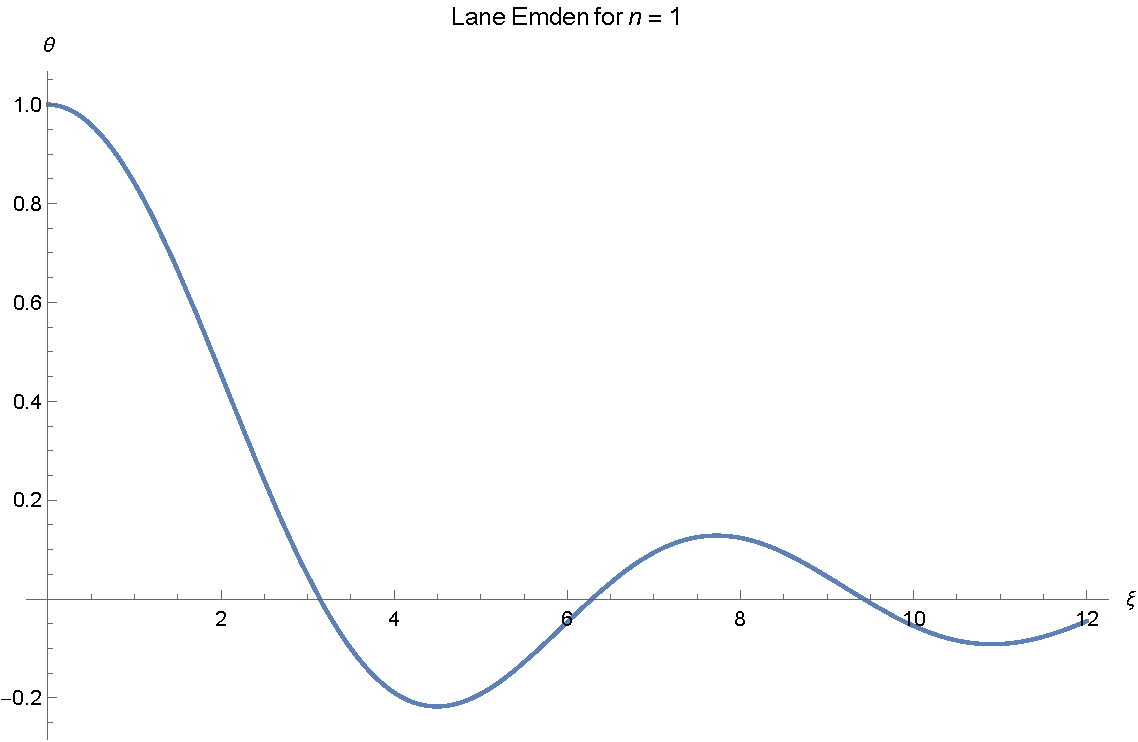
\includegraphics[width=1.0\linewidth]{Figures/n1solution}
	\caption{Solution to the Lane-Emden Equation for n=1}
	\label{fig:n1solution}
\end{figure}

From the substitution that we made, we know that $ \theta = 0 \iff \rho=0 $. We expect pressure to be zero hence, density to be zero at the surface i.e. $P(R) = \rho(R) = 0$ where $R$ is the radius of the star. Therefore we can write $ \theta(\xi_n) = 0 $ where $ \alpha \xi_n =R $. Then we can write the the total mass $M$ as
\begin{align}
	M = \int_{0}^{R} 4\pi r^2 \rho(r) dr = \int_{0}^{\xi_n} 4\pi\alpha^3\rho_c \xi^2 \theta^n(\xi) d\xi
\end{align}
Using Eq.\ref{Lane} we can substitute $\theta^n$ and easily evaluate the integral
\begin{align}\label{Mass}
	M =& -4\pi\alpha^3\rho_c\int_{0}^{\xi_n}\nonumber \dfrac{d}{d\xi}\bigg(\xi^2\frac{d\theta}{d\xi}\bigg)d\xi\\
	=&4\pi\alpha^3\rho_c(-\xi_n^2\theta'(\xi_n))\nonumber\\
	=& 4\pi R^3 \rho_c \bigg(\frac{\theta'(\xi_n)}{\xi_n}\bigg)
\end{align}
So, we derived the total mass $M$(Eq.\ref{Mass}) and we have an expression for $R$ (Eq.\ref{R}). Using these expressions and eliminating the $\rho_c$ in both expression we relate the mass and the radius of stars
\begin{align}\label{M-R}
	M = BR^{\frac{3-n}{1-n}}
\end{align}
where $B = 4\pi\bigg(\frac{K}{G} \frac{n+1}{4\pi}\bigg)^{n/n+1} \xi_n^{1+n/n-1} (-\theta'(\xi_n))$.

Since WDs are extremely dense objects their pressure is dominated by a quantum mechanical effect named electron degeneracy. Therefore EOS for cold WDs are give by
\begin{align}\label{EOS2}
	P =& C [ x(2x^2-3)(x^2+1)^{1/2} + 3sinh^{-1}x]
\end{align}
where $ x = \big(\frac{\rho}{D}\big)^{\frac{1}{q}} $. We cannot use \textit{Lane-Emden Equation} for these kind of stars. However, we can follow the same procedure and find an equation, modified version of \textit{Lane-Emden Equation} called \textit{Chandrasekhar White Dwarf Equation}.

\subsection{Chandrasekhar White Dwarf Equation}
We have the Hyrdrostatic Equlibrium Equation for a star(Eq.\ref{ODEs}) and the relation between the density and the pressure(Eq.\ref{EOS2}), therefore, we substitute pressure in the Hyrdrostatic Equlibrium Equations
\begin{align}
	\frac{1}{r^2}\frac{d}{dr}\bigg(\frac{d\sqrt{x^2 + 1}}{dr}\bigg) = - \dfrac{\pi G D^2}{2C}x^3 \nonumber
\end{align}
we define $y^2 = x^2 + 1$ and denote $ \rho_c = Dx_c^3 = D (y_c^2 - 1)^{3/2}$. Also we define
\begin{align}
	r = \beta \eta
\end{align}
where $ \beta = (\frac{2C}{\pi G D^2})^{1/2} \frac{\eta}{y_c} $ and finally we define $y = y_c \phi $. Then the equation reduces to
\begin{align}\label{Chandrasekhar WD}
	\frac{1}{\eta^2}\frac{d}{d\eta}\bigg(\eta^2 \dfrac{d\phi}{d\eta}\bigg) + (\phi^2 - \frac{1}{y_c^2})^{3/2} =0
\end{align}
which is called \textit{Chandrasekhar White Dwarf Equation}. The initial conditions are similar to Lane-Emden. We have $\phi(0) = 1$ and $\phi'(0) = 0$ but at the surface $ R=\beta\eta_n $ we have $\phi'(\eta_n) = \frac{1}{y_c^2}$.
\subsection{M-R curve}
We plotted the M-R points in figure \ref{fig:m-r-data} using the given data\footnote{whitedwarfdata.csv}. 
\begin{figure}
	\centering
	\includegraphics[width=1.0\linewidth]{"Figures/M-R data"}
	\caption{M-R for given data}
	\label{fig:m-r-data}
\end{figure}
Then, for the law mass stars i.e for $x\ll1$, using Mathematica\footnote{NewtonPartB.nb} we showed that Eq.\ref{EOS2} becomes
\begin{align}\label{EOS3}
	P = K_*\rho^{ 1 + \frac{1}{n_*}}
\end{align}
where $K_* = \frac{8C}{5D^{5/q}}$ and $n_* = q/(5-q)$. Therefore, we can now use Lane-Emden and Eq.\ref{M-R}. We made a fit to the data(figure\ref{fig:fit-to-m-r-low-mass}) and obtain the following values(in SI units) using Eq\ref{M-R}.
\begin{align}
	K_* &= 3144530.473379261\nonumber\\
	n_* &= 1,458045791\nonumber\\
	q &\approxeq 2.96 \nonumber
\end{align}
But we know from theory that q is an integer. Hence in order to make q an integer (i.e $q = 3$) we take $n = 1.5$.
\begin{figure}\label{fit}
	\centering
	\includegraphics[width=1.0\linewidth]{"Figures/fit to M-R (low mass)"}
	\caption{fit to M-R data for low mass stars}
	\label{fig:fit-to-m-r-low-mass}
\end{figure}
Since we know the index $n$ we can now solve the Lane Emden equation. For $n=1.5$ solution to the Lane-Emden(figure\ref{fig:solution-for-n1}) gives
\begin{figure}\label{n=1.5}
	\centering
	\includegraphics[width=1.0\linewidth]{"Figures/n15 lane emden"}
	\caption{Solution to the Lane-Emden for n =1.5}
	\label{fig:solution-for-n1}
\end{figure}
\begin{align}
\xi_n &= 3.653680580580581 \nonumber \\
\theta'(\xi_n) &= -0.20308599225966426\nonumber
\end{align}
Since we know the $ \xi_n $ and $ \theta'(\xi_n) $ we calculated the density of the center of the star $\rho_c$ for each pair of $R-M$ using Eq \ref{Mass}(Figure\ref{fig:rhoc-m-curve}).
\begin{figure}
	\centering
	\includegraphics[width=1.0\linewidth]{"Figures/rho_c-mass"}
	\caption{Mass-$\rho_c$ curve for low mass WDs}
	\label{fig:rhoc-m-curve}
\end{figure}

We found the parameter $n$ and the relation between $C$ and $D$ from the low mass fit for Eq\ref{EOS2}. So, we have only one unknown parameter $D$. To find the correct value of $D$ we did the following: We first start with an initial guess of $D = 1.7\times 10^9$ looking at the figure(\ref{fig:rhoc-m-curve}) and the fact that $x = (\rho/D)^{1/3} \ll 1$ for low mass stars and rise up to unity for others. For this initial guess we chose 20 random $rho_c$ values that will cover the whole $R$ range in our data. Using the $K$ value found we calculated the value of C. Then, with all the parameters we solved the \textit{Chandrasekhar's WD Equation(Eq.\ref{Chandrasekhar WD})}. From the solutions we calculated the corresponding $R$ and $M$ values, interpolated them using \textit{spline} from scipy and calculated the error from the original data. We repeated the same procedure for different values of $D$ to find the optimum value that minimizes the error. Eventually, we found the $ D $ and corresponding $ C $ with an error $ 2.1075048042135396\times10^{-9} $ as
\begin{align}
	C &= 5.380892404212922\times 10^{21}  \\
	D &= 1830000000.0\nonumber\\
	K &= 3144530.473379261\nonumber
\end{align} 
where the theoratical values of $ C $ and $ D $ is given as
\begin{align}\label{theoratical}
	C &= \dfrac{m_e^4c^5}{24\pi^2\hbar^3} = 6.002332114024319\times 10^{21}\\
	D &= \dfrac{m_u m_e^3c^3\mu_e}{3\pi^2 \hbar^3} = 1947865435.2624369\nonumber\\
	K &= 3161125.6038212245\nonumber
\end{align}
\subsection{Chandrasekhar Mass Limit}
Since we have all the parameters, we plotted the whole M-R curve(figure\ref{fig:full-m-r})
\begin{figure}
	\centering
	\includegraphics[width=1.0\linewidth]{"Figures/full M-R"}
	\caption{M-R curve for WDs}
	\label{fig:full-m-r}
\end{figure}
As can be seen in plot(figure\ref{fig:full-m-r}) there is a maximum mass allowed for WDs called \textit{Chandrasekhar Mass Limit}. We approximately calculated the value.\footnote{Chandrasekhar.py}. We started with some random $\rho_c$ values. Then we calculated the corresponding mass for each $\rho_c$. Then we saw that as we increase the $\rho_c$ we got a NS with a higher mass. So each time we increase the $\rho_c$ we calculated the difference between the last two masses and we saw that the difference is converging to zero as expected and highest mass value converges to some number that is found as
\begin{align}
	M_{Ch} =  1.3178477203482308 M_\odot
\end{align}
We also plotted the convergence of this calculation in figure(\ref{fig:convergence})
\begin{figure}
	\centering
	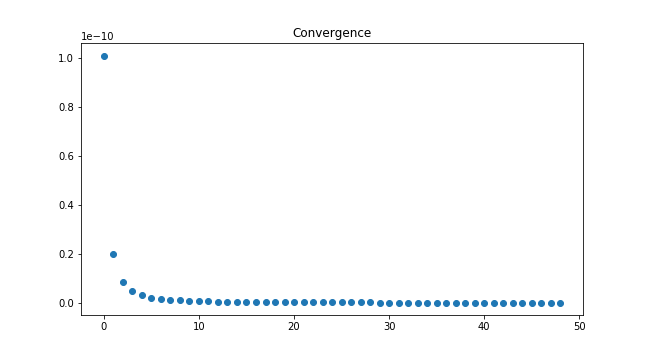
\includegraphics[width=1\linewidth]{Figures/convergence}
	\caption{Convergence of the Highest Mass Limit}
	\label{fig:convergence}
\end{figure}
We can also theoretically calculate this limit. Using Mathematica\footnote{mathematica folder} we showed that for $x \gg 1$ the Eq\ref{EOS2} becomes
\begin{align}
	P = 2Cx^4 + \dots
\end{align}
or since we know that $q = 3$
\begin{align}
	P = K\rho^{\frac{4}{3}} \implies n = 3
\end{align}
where $K = \frac{2C}{D^{4/3}}$. Then Using Equation \ref{M-R} we can find the Chandrasekhar Mass Limit for WDs as
\begin{align}
	M_{Ch} &= B = 4\pi\bigg(\frac{K}{G\pi}\bigg)^{3/2}\xi_3^2 (-\theta'(\xi_3))\\
\end{align}
If we put the constants from Eq.\ref{theoratical} as well as the solution of the Lane-Emden equation for n=3 which are found as $\xi_3 = 6.926992292292292$ and $\theta'(\xi_3) = -0.04210902023243969$ we found the Chandrasekhar Mass as
\begin{align}
	M_{Ch} = 1.45832101520284 M_\odot
\end{align}
Which is relatively close to what we found.

%%%%%%%%%%%%%%%%%%%%%%%%%%%%%%%%%%%%%%%%
%%%%%%%%%%%%%%%%%%%%%%%%%%%%%%%%%%%%%%%%
\section{Einstein}
%%%%%%%%%%%%%%%%%%%%%%%%%%%%%%%%%%%%%%%%
%%%%%%%%%%%%%%%%%%%%%%%%%%%%%%%%%%%%%%%%
We know that there is a mass limit for WDs and we calculated the value of it. Existence of such a limit brings the question: "what would happen if we try to add even more mass to WD?". The solutions we obtain so far was for WD at equilibrium. If a WD goes out of equilibrium it starts to collapse and instability continuous  until some other mechanism takes place. Sometimes these collapses can end up in big explosions and destruction of WDs called \textit{Type Ia supernova} explosions. And sometimes WD squeezes so much that electrons and protons merges and creates neutrons. If the electron degeneracy pressure can obtain stability, a star made of mostly neutrons  emerges. These stars called as Neutron Stars (NS). NS usually have a radius around 10-20 km and a few solar mass. Therefore gravity becomes so immense that we can no longer use the Newton's Equations, instead we use Einstein's General Relativity.

We can expect NS to behave like WD but with a non-interacting electron model, however, neutrons in NS interacts with each other. In fact, the interaction are so complicated that we don't know the exact EOS. Therefore, for simplicity we will use 
\begin{align}\label{EOS NS}
	P = K_{NS}\rho^2
\end{align}
which gives qualitative behavior of NSs. And for Simplicity we take $ K =50 $

From now on, we will use the geometric units i.e. $ M_\odot $ as the mass unit, $ \frac{GM_\odot }{c^2} \approx 1477m$ as length unit and $ \frac{GM_\odot }{c^3} \approx 4.927\times10^{-6}s$ as time unit so that $c = G = 1$. 

\subsection{Tolman-Oppenheimer-Volkoff (TOV) Equations}
Hydrostatic equilibrium equations are modified due to general relativistic effects are called Tolman-Oppenheimer-Volkoff (TOV) Equations and given as:
\begin{align}\label{TOV}
	m' &= 4\pi r^2 \rho\\
	\nu' &= 2\frac{m + 4\pi r^3p }{r(r-2m)}\nonumber\\
	p' &= - \frac{1}{2}(\rho + p )\nonumber\nu' 
\end{align}
where ' indicates the derivative w.r.t $ r $ and $e^{\nu(r)/2}$ is the time dilation factor of relativity. We solve this system of ODEs just as in Newtonian case. We will stop when $p =0 \iff \rho = 0$ with initial conditions $m(0) = 0 $ and $ p(0) = p_c$ or $\rho(0) = \rho_c$. And by definition, $e^{v(0)/2}$ is the time dilation factor due to gravity at the center of the star compared to an observer at $ r\rightarrow \infty $. So we need to start with $ \nu(0) $ that gives $ \mu(\infty) = 0 $. We cannot know this in advance but it does not matter. Because adding a constant to $ \mu $ does not effect the solution of $ m(r) $ and $ p(r) $. Therefore we will simply use $ \mu(0) = 0 $. 

We obtained the $ M-R $ curve(figure \ref{fig:mass-radius-of-neutron-stars}) by solving Eqs\ref{TOV} for different $p_c$'s. 

\begin{figure}
	\centering
	\includegraphics[width=1.0\linewidth]{"Figures/Figures_Einstein/Mass-Radius of Neutron Stars"}
	\caption{M-R curve for NSs}
	\label{fig:mass-radius-of-neutron-stars}
\end{figure}

But, the $m(r)$ functions that we calculated is actually not the rest mass of the stars. Since mass is the energy in relativity and gravitational potential energy is negative; what we calculated contains the rest mass as well as negative contribution due gravity. Therefore, in order to find the rest mass which is called \textit{baryonic mass} we need to solve the following ODE
\begin{align}\label{baryonic}
	m_P' = 4\pi\bigg(1 - \frac{2m}{r})^{-1/2} r^2\rho
\end{align}
And we define the fractional binding energy  as
\begin{align}\label{fractional}
	\Delta \equiv \frac{M_P - M}{M}
\end{align}
We plotted Gravitational potential energy $\Delta$ vs Radius $R$ in figure \ref{fig:fractional-binding-energy-of-neutron-stars}
\begin{figure}
	\centering
	\includegraphics[width=1.0\linewidth]{"Figures/Figures_Einstein/Fractional Binding Energy of Neutron Stars"}
	\caption{Fractional Binding Energy - Radius curve of Neutron Stars}
	\label{fig:fractional-binding-energy-of-neutron-stars}
\end{figure}

\subsection{Stability of Neutron Stars}
Stability condition for a NS is give as
\begin{align}\label{stability}
	\frac{dM}{d\rho_c} &> 0 \rightarrow stable\\
	\frac{dM}{d\rho_c} &< 0 \rightarrow unstable \nonumber
\end{align}
The reason behind these conditions are as follows. If we squeeze the star a little bit, a stable star resist this process since it is stable. Therefore we do positive work which means mass increases since mass is energy in relativity. Density also increases but overall $ \frac{dM}{d\rho_c} > 0 $. If star is unstable it continuous squeezing since it already wants to go to a lower energy level. It continuous doing this till it finds a stable equilibrium or forms a black hole. 

Therefore we plotted the $\rho_c vs M$ curve(figure \ref{fig:rhoc---mass-of-neutron-stars}) to and find the stability region for the NSs.
\begin{figure}
	\centering
	\includegraphics[width=1.0\linewidth]{"Figures/Figures_Einstein/rho_c - mass of Neutron Stars"}
	\caption{$\rho_c vs M$ Curve}
	\label{fig:rhoc---mass-of-neutron-stars}
\end{figure}
Then by looking for the conditions in Eq.\ref{stability} we conclude where the NSs are stable and where they are unstable. We plotted to M-R curve and indicate which NSs are stable in figure \ref{fig:stability-of-neutron-stars}. Also we conclude that there is a maximum mass $M_{max}$ allowed by this EOS. From figure \ref{fig:stability-of-neutron-stars} or figure \ref{fig:mass-radius-of-neutron-stars} we found this value by looking at where the derivative zero with a tolerance $10^{-21}$\footnote{{MRcurveforNS.py}}. The found value is
\begin{align}\label{maxM}
	M_{max} = 1.410421107619103  M_\odot
\end{align}

\begin{figure}
	\centering
	\includegraphics[width=1.0\linewidth]{"Figures/Figures_Einstein/stability of Neutron Stars"}
	\caption{Stability of NSs}
	\label{fig:stability-of-neutron-stars}
\end{figure}

\subsection{Maximum K value for Neutron Stars}

We take $ K=50 $ at the beginning of our calculations and find the $ M_{max} $(\ref{maxM}). And we know that maximum mass observed for a NS is $ 2.14M_\odot $. Therefore there is maximum value for $K = K_{max}$. To find this value we plotted the maximum mass values $M_{max}$ for different $K$(figure). From the curve it can be seen that around maximum mass $ 2.14M_\odot $ we have the K value as
\begin{align}
	K_{max} \approx 239
\end{align}
\begin{figure}
	\centering
	\includegraphics[width=1\linewidth]{"Figures/Figures_Einstein/Max Mass - K"}
	\caption{$M_{max} - K curve$}
	\label{fig:max-mass---k}
\end{figure}

Since there is no matter outside the star we modify equation \ref{TOV}. Outside the star i.e $r>R$ we have $m(r>R) = M$ also we have $p(r>R) = 0$. Then equation for $\nu(r)$ becomes
\begin{align}
	\nu' = \frac{2M}{r(r-2M)}
\end{align}
Using Mathematica we showed that this integration simply gives
\begin{align}\label{mu}
	\mu(r>R) = \ln\bigg( 1 - \frac{2M}{r} \bigg) - \ln\bigg( 1 - \frac{2M}{R} \bigg) + \nu(R) 
\end{align}
And as we mention we can shift $\nu$ by a constant. Since we want $ e^{\nu(\infty)} = 1 $ i.e. no time dilation for an observer at infinity, we can simply remove the constant terms from Eq\ref{mu} which yields
\begin{align}
	\bar{\nu}(r>R) = \bigg(1 - \frac{2M}{r}\bigg) 
\end{align}
which also satisfies $ e^{\bar{\nu}(\infty)} = 1 $.

%%%%%%%%%%%%%%%%%%%%%%%%%%%%%%%%%%%%%%%%
%%%%%%%%%%%%%%%%%%%%%%%%%%%%%%%%%%%%%%%%
\section{Beyond Einstein}
%%%%%%%%%%%%%%%%%%%%%%%%%%%%%%%%%%%%%%%%
%%%%%%%%%%%%%%%%%%%%%%%%%%%%%%%%%%%%%%%%

\subsection{Wave Equation}
A massless real Klein Gordon field obeys the wave equation
\begin{align}
	\square\phi = 0 \implies \bigg(-\frac{\partial^2}{\partial t^2}\bigg)
\end{align}
If we assume spherical symmetry and if we are interested in space-time of a NS Modified Wave equation in curved spacetime becomes
\begin{align}
	square\phi &= 0\nonumber\\
	&= -\frac{1}{\sqrt{|g(r)|}} \frac{\partial}{\partial t} \bigg[
	e^{-\bar{\nu}\sqrt{|g(r)|}} \frac{\partial \phi}{\partial t}
	\bigg]\nonumber\\
	&+ \frac{1}{\sqrt{|g(r)|}} \frac{\partial}{\partial r} \bigg[\bigg(1 - \frac{2m(r)}{r}\bigg)\sqrt{|g(r)|} \frac{\partial \phi}{\partial r}\bigg]
\end{align}
We reduce this equation to first order as follows
\begin{align}
	\partial_t \Phi = \partial_r (f(r) \Pi)\\
	\partial_t \Pi = \frac{1}{r^2}\partial_r(r^2f(r)\Phi)
\end{align}
where we defined 
\begin{align}
	\Phi &\equiv \partial_r\phi\\
	\Pi &\equiv  \frac{1}{f(r)}\partial_t\nonumber\\
	f(r) &\equiv e^{\bar{\nu}(r)/2} \bigg(1 - \frac{2m(r)}{r}\bigg)^{1/2}\nonumber
\end{align}
In order to have a smooth physical solutions we need to impose the following boundary conditions
\begin{align}
	\Phi(0) = \partial_r\Pi = 0\\
	\lim\limits_{r \rightarrow \infty }\Phi \rightarrow \frac{1}{r}\\
	\lim\limits_{r \rightarrow \infty }\Pi \rightarrow \frac{1}{r}
\end{align}
with the following initial conditions
\begin{align}
	\phi(0,r) &= 10^{-3}e^{-r^2/2}\\
	\dot{\phi}(0,r) &= 0 
\end{align}
We discretize the domain using Leap-Frog Scheme for advection equation.
\begin{align}
	\Phi_j^{n+1} &= \Phi_j^{n-1} + \lambda ((f_{j+1}\Pi_{j+1}^n ) - (f_{j-1}\Pi_{j-1}^n ))\\
	\Pi_{j}^{n+1} &= \Pi_j^{n-1} + \lambda g_j((\frac{1}{g}f\Phi)^n_{j+1} - (\frac{1}{g}f\Phi)^n_{j-1})\label{leapfrog}
\end{align}

Then just by using Implicit Euler Method we calculated the $\phi$
\begin{align}
	\phi_{j+1}^n = \phi_{j}^n  + \Delta r\Phi^n_{j+1}
\end{align}
Then, we plotted the wave $ \phi(t,r) $ to see how it evolves in time in figure \ref{fig:waveequation}. As can be seen, the initial wave changes its amplitude as it moves. It decreases and increases again
\begin{figure}
	\centering
	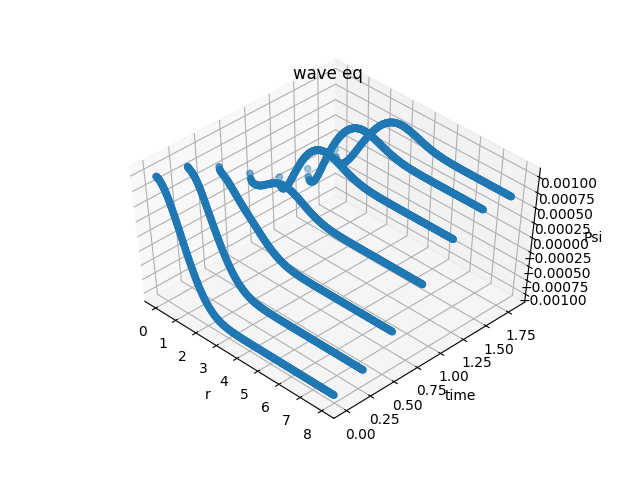
\includegraphics[width=1\linewidth]{Figures/Beyond_Einstein_Figures/wave_equation}
	\caption{Solution to wave equation $ \phi(t,r) $ }
	\label{fig:waveequation}
\end{figure}

In a certain class of alternative theories of gravity named scalar-tensor theories, the wave equation for the scalar is modified as
\begin{align}\label{modified eq}
	\square\phi = 4\pi\beta e^{ 2\beta\phi^2}(\rho- 3p)\phi
\end{align}
Therefore we modified our Leap-frog scheme in equation\ref{leapfrog}
\begin{align}
		\Pi_{j}^{n+1} = \Pi_j^{n-1} + \lambda g_j((\frac{1}{g}f\Phi)^n_{j+1} - (\frac{1}{g}f\Phi)^n_{j-1}) \\
		+ 48\pi e^{-12\phi_{j}^2}(\rho_j-3p_j)\phi_{j}^n\Delta t
\end{align}
and we got the following result
\begin{figure}
	\centering
	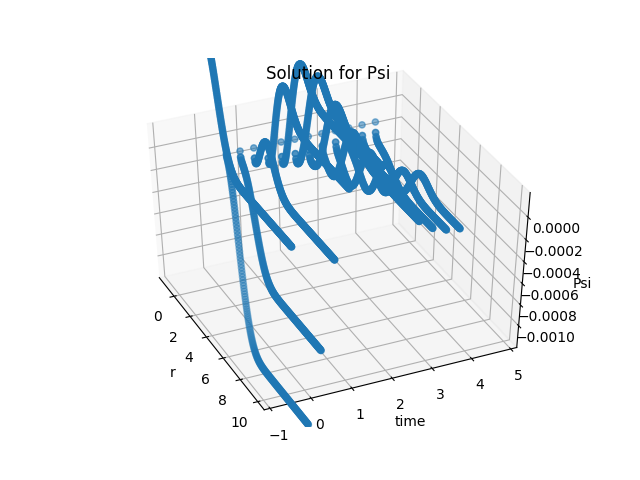
\includegraphics[width=1\linewidth]{Figures/Beyond_Einstein_Figures/wave_equation_termadded}
	\caption{Solution to wave equation $ \phi(t,r) $ with additional term}
	\label{fig:waveequationtermadded}
\end{figure}

\begin{figure}
	\centering
	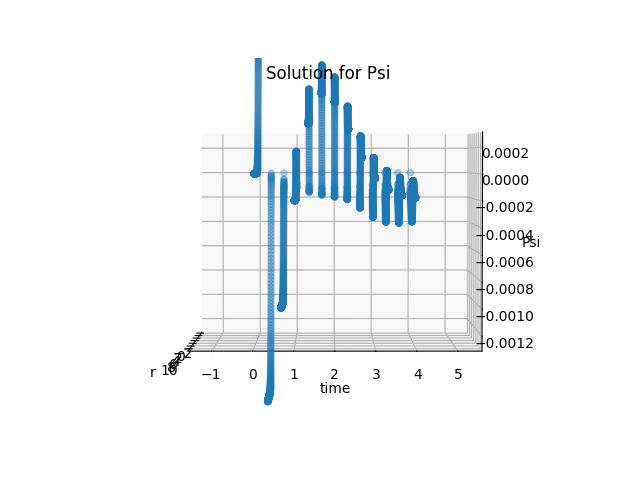
\includegraphics[width=1\linewidth]{Figures/Beyond_Einstein_Figures/wave_equation_termadded2}
	\caption{Side view of the figure \ref{fig:waveequationtermadded}}
	\label{fig:waveequationtermadded2}
\end{figure}
 As can be seen in plots, after adding the term in Eq.\ref{modified eq}, $\phi(t,r)$ grows and reaches an almost stable configuration not changing in time.
%%%%%%%%%%%%%%%%%%%%%%%%%%%%%%%%%%%%%%%%%%%%%%%%%%%%%%%%%%%%%%%%%%%%
%%%%%%%%%%%%%%%%%%%%%%%%%%%%%%%%%%%%%%%%%%%%%%%%%%%%%%%%%%%%%%%%%%%%

\textit{Acknowledgments: I would like to thank Fethi M\"{u}bin Ramazano\u{g}lu who taught me computational physics, helped me pushed my limits, gave me the opportunity to write this paper.  }
\bibliography{references} % the name of the file where you keep the references you cite.

\end{document}
